

%\documentclass{book}\begin{document}<content\end{document}
\documentclass[letter, 11pt, margins=0.3in]{texMemo}  % The texMemo package by Rob Oakes.

\usepackage{amsmath}
\usepackage{color, soul}
\usepackage{dcolumn}
    \newcolumntype{d}[1]{D{.}{.}{#1}}
\usepackage[colorlinks=true, citecolor=blue]{hyperref}
\usepackage{enumitem}
\usepackage{graphicx, lipsum}

\usepackage{caption}
\usepackage{subcaption}

\usepackage[LGRgreek]{mathastext}

\usepackage{listings}
\usepackage[]{matlab-prettifier}

\usepackage{multirow}

\usepackage{natbib}
\bibliographystyle{apalike}

\usepackage{printlen}  % \printlength\textwidth - To determine textwidth of document.  Here is it 496 pt.

\usepackage[table]{xcolor}
\definecolor{maroon}{cmyk}{0,0.87,0.68,0.32}
\definecolor{LightCyan}{rgb}{0.88,1,1}
\definecolor{Gray}{gray}{0.85}


\graphicspath{ {../} }


\memodate{\today~(Submitted)}
\memosubject{ACS 547, Noise Control Applications - Module 2 Assignment\\}



\begin{document}

\maketitle


\vspace{-0.25cm}
\section*{Problem 1 - Modal Behaviour of a Cylindrical Room}

The Matlab code for this problem is listed in Appendix~\ref{appendix:problem1}.

\vspace{0.25cm}
\subsection*{Problem 1a}

Table~\ref{table:resonanceFrequencies} lists the ten lowest resonance mode orders for the room and the respective frequency.

\setlength{\abovecaptionskip}{0pt}
\vspace{0.1cm}
{\renewcommand{\arraystretch}{1.5}
\begin{table}[h!]
    \begin{center}
        \small
        \begin{tabular}{ | c | c | c | }
            \hline
            \textbf{Index}  &  \textbf{Mode ($\mathbf n_x$, $\mathbf n_\theta$, $\mathbf n_r$)}  &  \textbf{Frequency [Hz]}  \\
            \hline
                0  &  0, 0, 0  &  0  \\
                \rowcolor{Gray}
                1  &  1, 0, 0  &  17.2  \\
                2  &  0, 1, 0  &  33.5  \\
                \rowcolor{Gray}
                3  &  2, 0, 0  &  34.3  \\
                4  &  1, 1, 0  &  37.6  \\
                \rowcolor{Gray}
                5  &  2, 1, 0  &  48.0  \\
                \rowcolor{pink}
                \hline
                6  &  3, 0, 0  &  51.5  \\
                \rowcolor{pink}
                \hline
                7  &  0, 2, 0  &  55.6  \\
                \hline
                8  &  1, 2, 0  &  58.2  \\
                \rowcolor{Gray}
                9  &  3, 1, 0  &  61.4  \\
                10  &  2, 2, 0  &  65.3  \\
            \hline
        \end{tabular}
    \end{center}
    \caption{Resonant modes of the cylindrical room.}
    \label{table:resonanceFrequencies}
\end{table}




\vspace{0.25cm}
\subsection*{Problem 1b}

The two closest modes are (3, 0, 0) and (0, 2, 0) with frequencies of 51.5 Hz and 55.6 Hz, respectively.




\vspace{0.25cm}
\subsection*{Problem 1c}

Figure~\ref{fig:modeVisualization} illustrates the (3, 0, 0) and (0, 2, 0) modes.  The white lines in each figure show the modal lines for that mode.  \textbf{The machine can be placed where the modal lines for each mode overlap}.  The figures were produced using the Room Eigenmode Simulator Version 1.1 software package.

\vspace{0.25cm}
The pink rings in Figure~\ref{fig:sub2} indicate 3 possible places where the machine could be placed.  These points coincide with the three modal planes shown in Figure~\ref{fig:sub1}.  Theoretically, there are an infinite number of places where the machine could be placed.  However, placement would take into account practical considerations such as accessibility, etc.


\begin{figure}[htbp]
    \centering
    \begin{subfigure}{0.5\textwidth}
        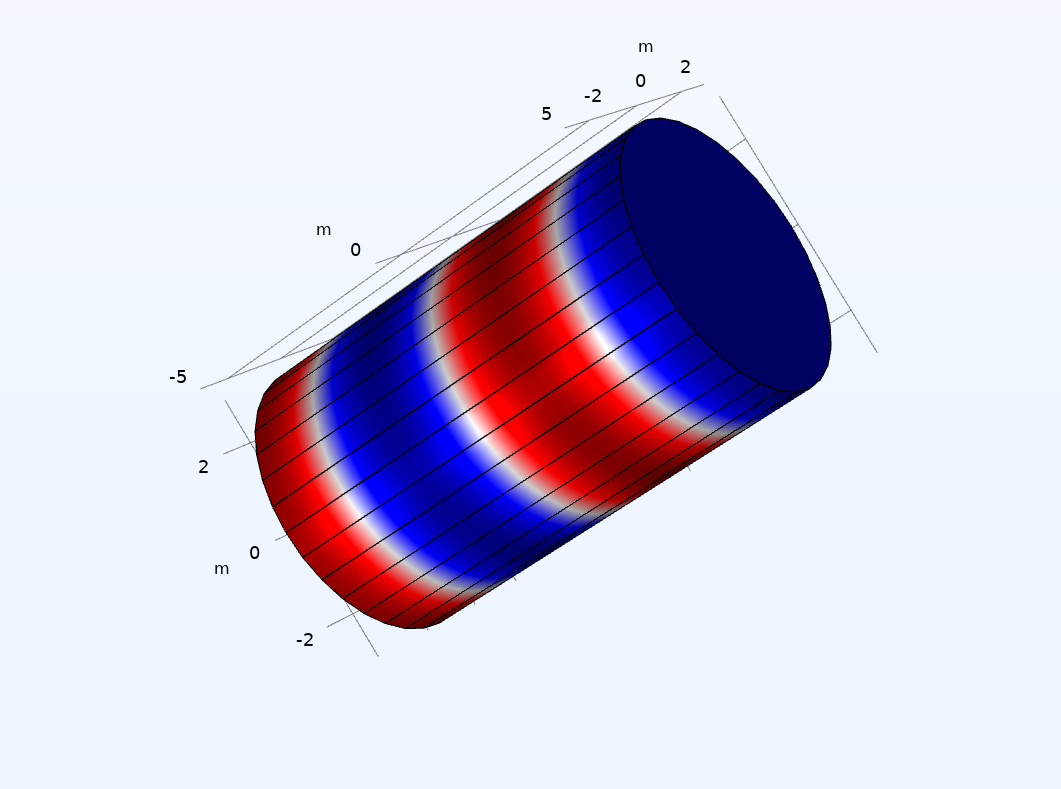
\includegraphics[width=\textwidth]{Mode Profile 51_5 Hz.png}
            \caption{Mode (3, 0, 0)}
            \label{fig:sub1}
    \end{subfigure}
    \vspace{0.25cm}
    \begin{subfigure}{0.5\textwidth}
        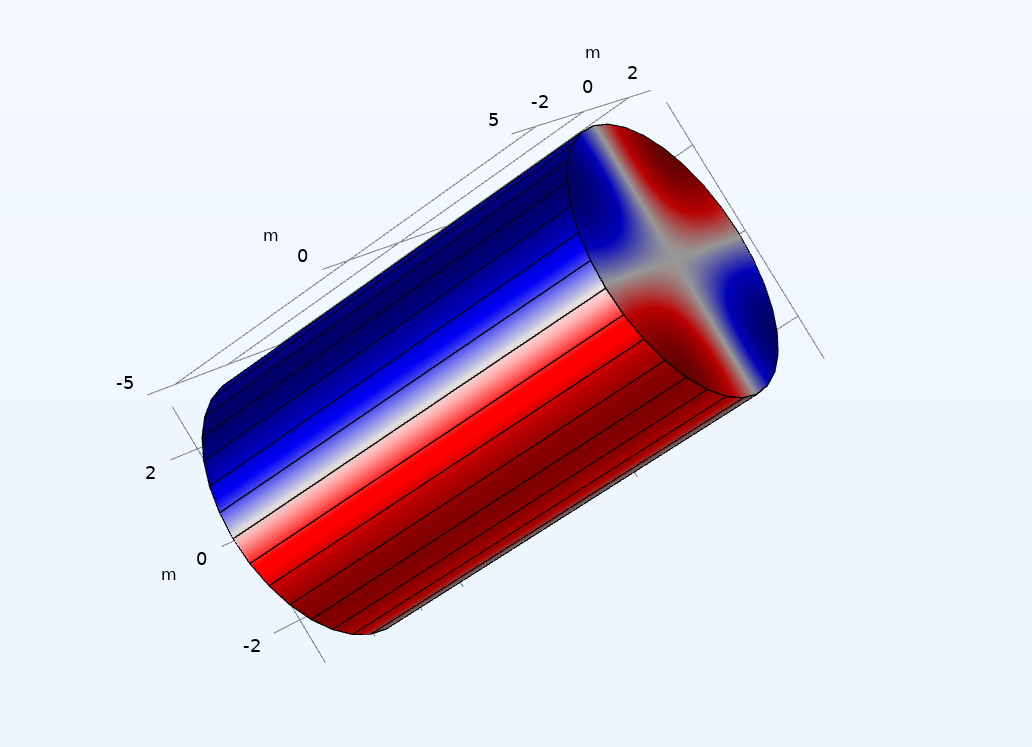
\includegraphics[width=\textwidth]{Mode Profile 55_8 Hz.png}
            \caption{Mode (0, 2, 0)}
            \label{fig:sub2}
    \end{subfigure}
    \vspace{0.5cm}
    \caption{Visualization of modes.  (a.) Mode (3, 0, 0).  (b.) Model (0, 2, 0).  The pink circles in~\ref{fig:sub2} illustrate a few modal line intersections where the machine could be placed.}
    \label{fig:modeVisualization}
\end{figure}






\newpage
\section*{Problem 2 - Sabine Room}

The Matlab code for this problem is listed in Appendix~\ref{appendix:problem2}.


\vspace{0.25cm}
\subsection*{Problem 2a}

The reverberant field sound pressure level is approximately 98.3 dB SPL.




\vspace{0.25cm}
\subsection*{Problem 2b}

Figure~\ref{figure:sabineRoomLevels} shows the direct, reverberant, and total sound pressure levels for a 25 mW, 125 Hz, broadband, omnidirectional source placed centrally in the room (i.e. the directivity factor is 1).

\vspace{-4cm}
\begin{figure}[htb!]
    \center
        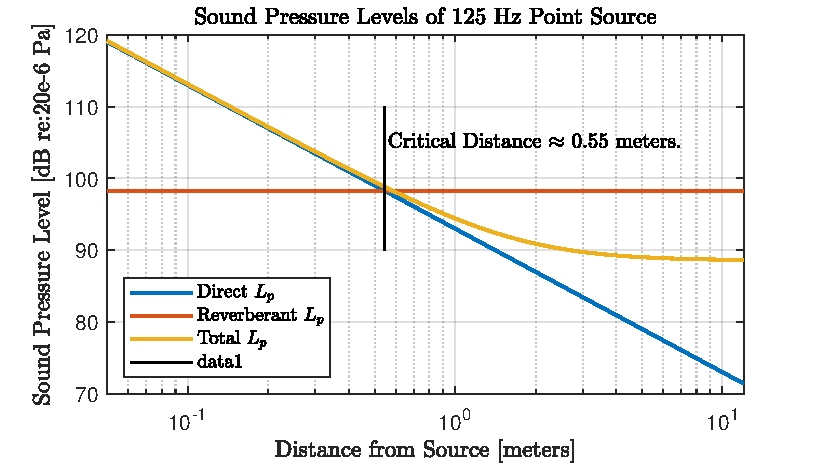
\includegraphics[ scale = 0.65, keepaspectratio ]{Sabine Room.pdf}
    \vspace{-3.5cm}
    \caption{Sound levels for the room produced by a 25 mW, 125 Hz omnidirectional, broadband source.}
    \label{figure:sabineRoomLevels}
\end{figure}






\newpage
\section*{Problem 3 - Transmission Loss Measurement}

The Matlab code for this problem is listed in Appendix~\ref{appendix:problem3}.

\vspace{0.25cm}
Figure~\ref{figure:q3AverageAbsorption} shows the average absorption per octave band based on the T60 data.  The calibration plate isolates the receiver room and the absorption calculation does not consider the calibration plate.


\begin{figure}[htb!]
    \center
        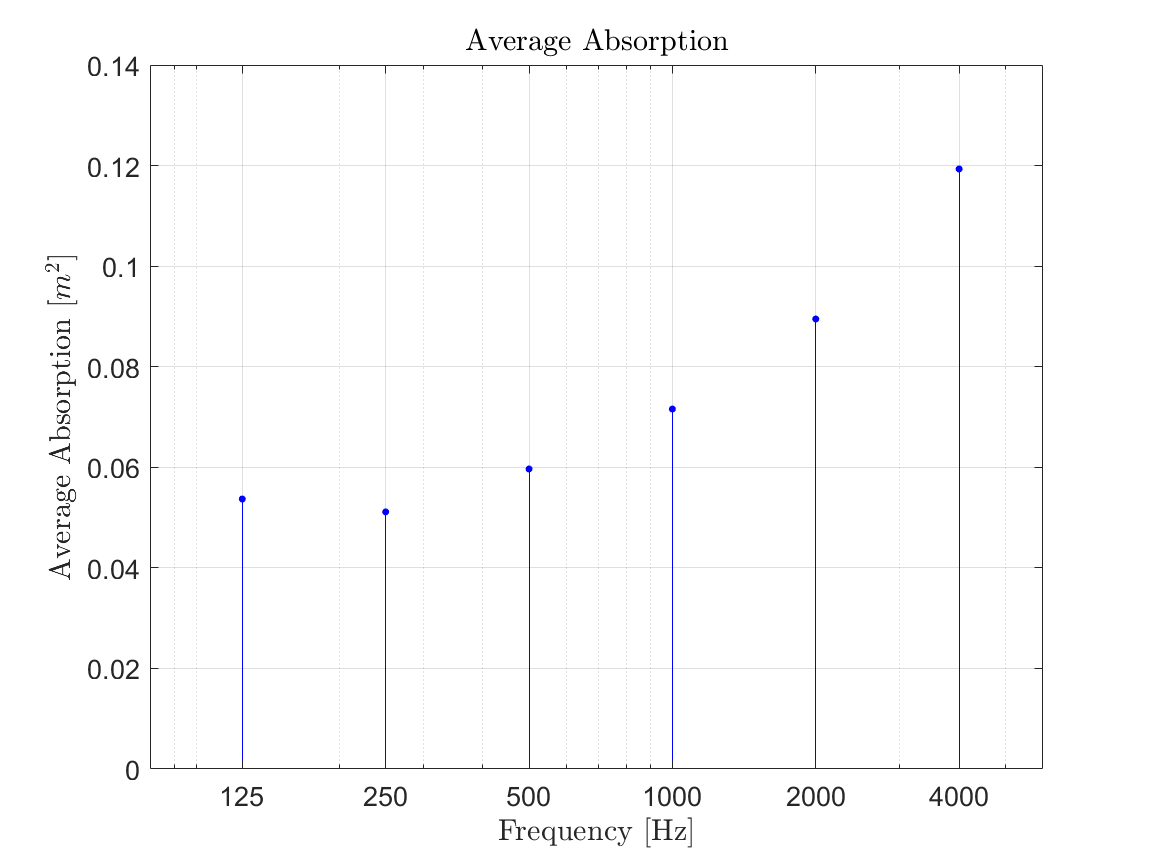
\includegraphics[ scale = 0.6, keepaspectratio ]{Q3 Average Absorption.png}
    \caption{Average absorption per octave band.}
    \label{figure:q3AverageAbsorption}
\end{figure}


\vspace{0.2cm}
Figure~\ref{figure:q3TransmissionLoss} shows the transmission loss per octave band.


\begin{figure}[htb!]
    \center
        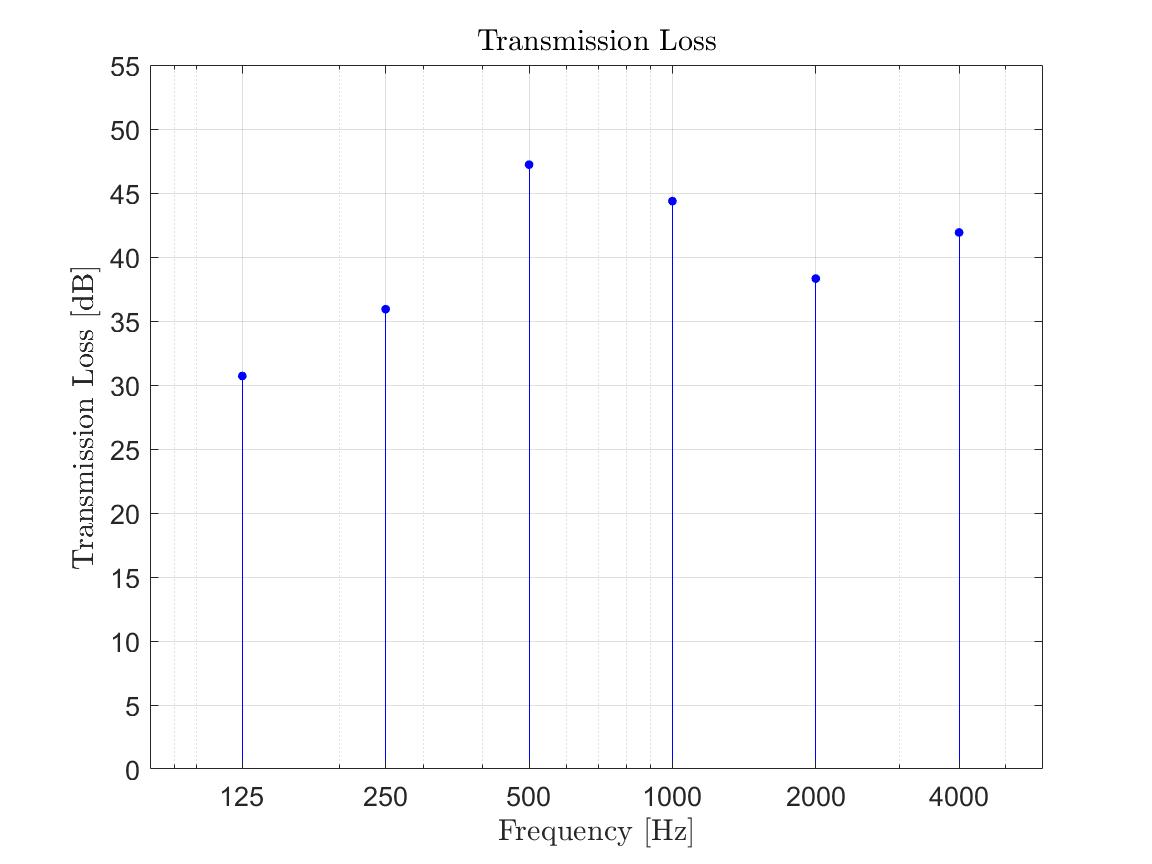
\includegraphics[ scale = 0.6, keepaspectratio ]{Q3 Transmission Loss.png}
    \caption{Transmission loss per octave band.}
    \label{figure:q3TransmissionLoss}
\end{figure}






\newpage
\section*{Problem 4 - Panel Transmission Loss}

The Matlab code for this problem is listed in Appendix~\ref{appendix:problem4}.

\subsection*{Problem 4a}

The resonance frequency, $f_o$, of the galvanized steel panel is 4 Hz or 22.6 $\frac{radians}{s}$.


\subsection*{Problem 4b}


\vspace{0.25cm}
\subsubsection*{i - Critical Frequency and Coincidence Frequency at 75$^\circ$}

The critical frequency is 10,216 $Hz$ and the coincidence frequency at 75$^\circ$ is 10,494 $Hz$.



\vspace{0.25cm}
\subsubsection*{ii - Transmission Loss at Angle of Incidence of 75$^\circ$}

Figure~\ref{figure:q4transmissionLossAt75} shows the transmission loss for an angle of incidence of 75$^\circ$.

\begin{figure}[htbp]
    \center
    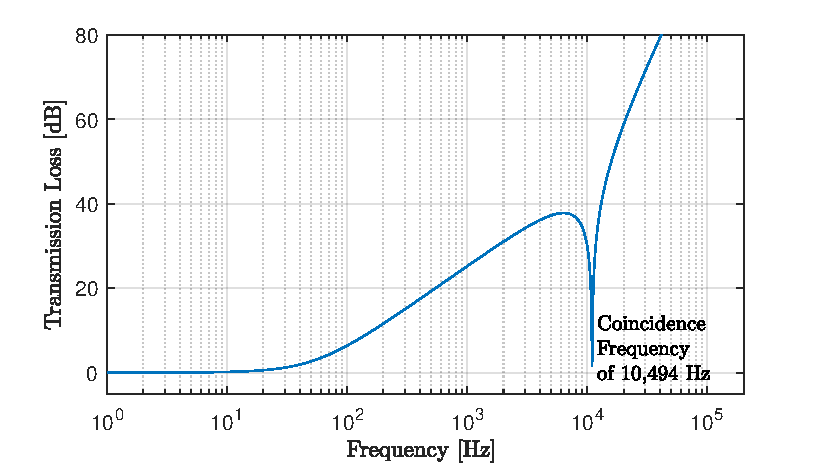
\includegraphics[scale=0.9]{Q4 TL for 75 AOI.pdf}
    \vspace{0.25cm}
    \caption{Flexible Panel Transmission Loss for a 75$^\circ$ Incidence Angle}
    \label{figure:q4transmissionLossAt75}
\end{figure}



\vspace{0.25cm}
\subsubsection*{iii - Transmission Loss for Angles of Incidence between 0-90$^\circ$}

Figure~\ref{figure:q4iiitransmissionLossAt75} shows the transmission loss angles of incidence from 0 to 90$^\circ$ in steps of 10$^\circ$.

\begin{figure}[htbp]
    \center
    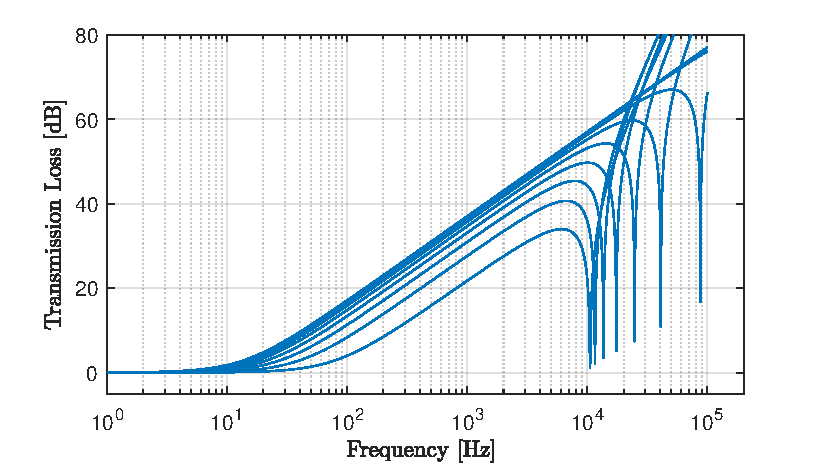
\includegraphics[scale=0.9]{Q4iii TL for 75 AOI.pdf}
    \vspace{0.25cm}
    \caption{Flexible Panel Transmission Loss for angles of incidence between 0 and 90$^\circ$.}
    \label{figure:q4iiitransmissionLossAt75}
\end{figure}



\vspace{0.25cm}
\subsubsection*{iv - Diffuse Transmission Loss}

See the Matlab code in the Appendix~\ref{appendix:problem4}



\newpage
\subsection*{Problem 4c}

See the Matlab code in the Appendix~\ref{appendix:problem4}



\subsection*{Problem 4d}

Figure~\ref{figure:q4dtransmissionLoss} shows the transmission loss angles of incidence from 0 to 90$^\circ$ in steps of 10$^\circ$.

\begin{figure}[htbp]
    \center
    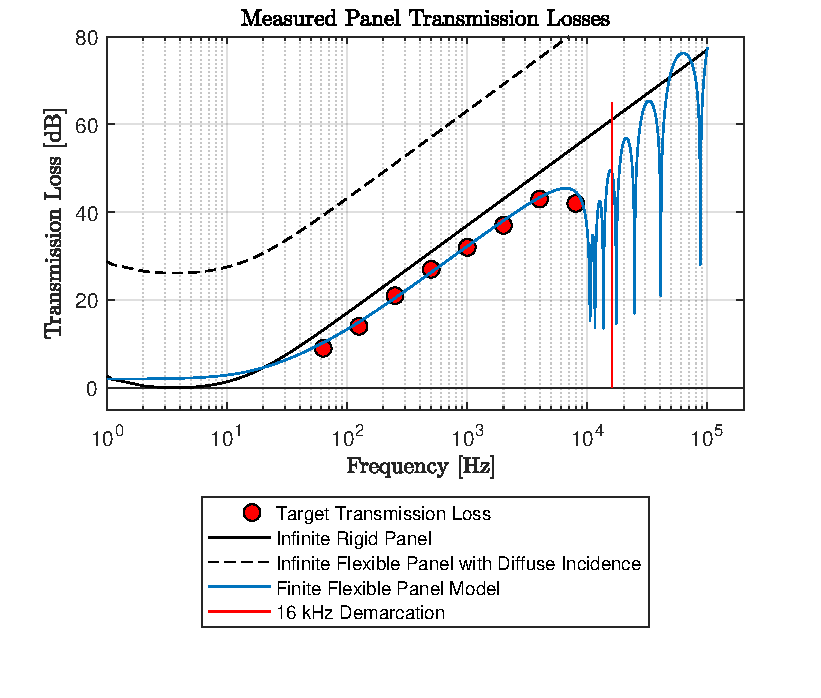
\includegraphics[scale=0.9]{Q4d TL for 75 AOI.pdf}
    \vspace{-0.5cm}
    \caption{Measured data and the modeled responses.}
    \label{figure:q4dtransmissionLoss}
\end{figure}

\textbf{The finite flexible panel appears to be the most appropriate model}.  As noted in class, the measured transmission loss at 8 kHz is smaller than the loss a 4 kHz.  This indicates that the loss at 16 kHz should be less than the response of the infinite rigid panel at 16 kHz.







\newpage
\section*{Problem 5 - Large Enclosure Design}

The Matlab code for this problem is listed in Appendix~\ref{appendix:problem5}.

\vspace{0.25cm}
My enclosure is a 2 $m$ cube that sits on the ground (5 sides of enclosure material) over the machine.  The machine is suspended above the pad (directivity factor of unity).  It is assumed that there is no noise transmission through the ground.

\vspace{0.25cm}
Table~\ref{table:targetInsertionLosses} lists the target insertion losses, the calculated insertion losses for four materials, and the loss difference between the target and each type of material.  \textit{A positive value indicates that the target insertion loss for the given octave band was not met}.

\vspace{0.25cm}
Figure~\ref{figure:q5ilPlot} shows calculated insertion loss differences for the data in Table~\ref{table:targetInsertionLosses}.

\vspace{0.25cm}
\setlength{\abovecaptionskip}{0pt}
\vspace{0.1cm}
{\renewcommand{\arraystretch}{1.25}
\begin{table}[h!]
    \begin{center}
        \small
        \begin{tabular}{ | c | c | c | c | c | c |}
            \hline
            \textbf{Octave Band [Hz]}  &  \textbf{Target IL [dB]}  &  \textbf{QBV 2 [dB]}  &  \textbf{QBV 3 [dB]}  &  \textbf{HTL (100MM) [dB]}  &  \textbf{HTL 4 [dB]}  \\
            \hline
            250    &  44  &  28.0  &  19.7  &  10.6   &  5.6  \\
            \rowcolor{Gray}
            500    &  54  &  26.7  &  22.2  &  6.6    &  -4.4  \\
            1,000  &  45  &  5.6   &  1.4   &  -15.4  &  -22.4  \\
            \rowcolor{Gray}            
            2,000  &  47  &  -8.4  &  -2.2  &  -18.4  &  -19.4  \\
            4,000  &  58  &  -2.4  &  5.7   &  -11.0  &  -13.0  \\
            \hline
        \end{tabular}
    \end{center}
    \caption{Calculated insertion losses for the 4 enclosure materials.}
    \label{table:targetInsertionLosses}
\end{table}

\vspace{-0.5cm}
\begin{figure}[htbp]
    \center
    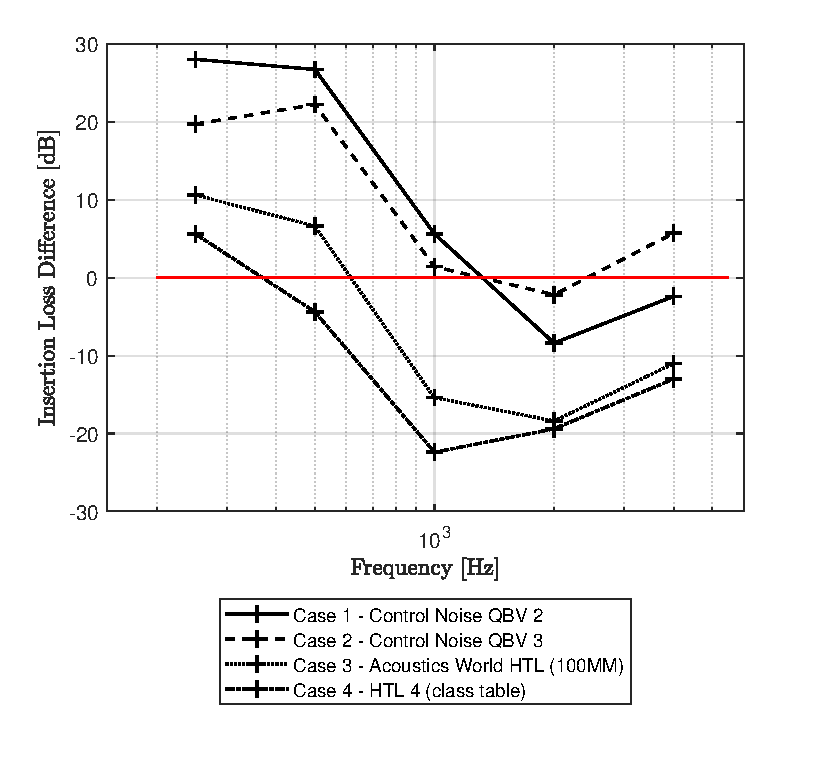
\includegraphics[scale=0.8]{Q5 IL Plot.pdf}
    \vspace{-0.5cm}
    \caption{Insertion loss differences.}
    \label{figure:q5ilPlot}
\end{figure}

The most restrictive case given the 2 cubic-meter, 5-sided enclosure, is the HTL 4 material, Case 4, which was presented in class.  The target insertion loss was reached by all of the octave bands except the 250 Hz band.

\vspace{0.25cm}
With the same enclosure dimensions and machine orientation, the HTL (100MM) material, Case 3, was found to be the second best material, not meeting the 250 Hz and 500 Hz targets. Figure~\ref{figure:q5AWcaseData} shows the transmission loss and absorption coefficient data for the material selected from \href{https://www.acousticsworld.com/machine-acoustic-enclosures/}{Acoustics World}.

\vspace{0.25cm}
The QBV-2 and QBV-3 , Case 1 and Case 2, respectively, had the poorest performance.  
Figure~\ref{figure:q5CNcaseData} shows the transmission loss and absorption coefficient data for these material from 
\href{https://www.controlnoise.com/wp-content/uploads/2022/02/Acoustic-Enclosures-Datasheet.pdf}{Control Noise}.

\vspace{0.25cm}
Using the HTL 4 material from class, a cube with 2 $m$ sides appeared to produce the optimal insertion loss for the 250 Hz octave band.  Making the size of the enclosure larger does not reduce this insertion loss and does not seem to be practical.  A supplementary approach for this octave band should be considered.

\begin{figure}[htbp]
    \center
    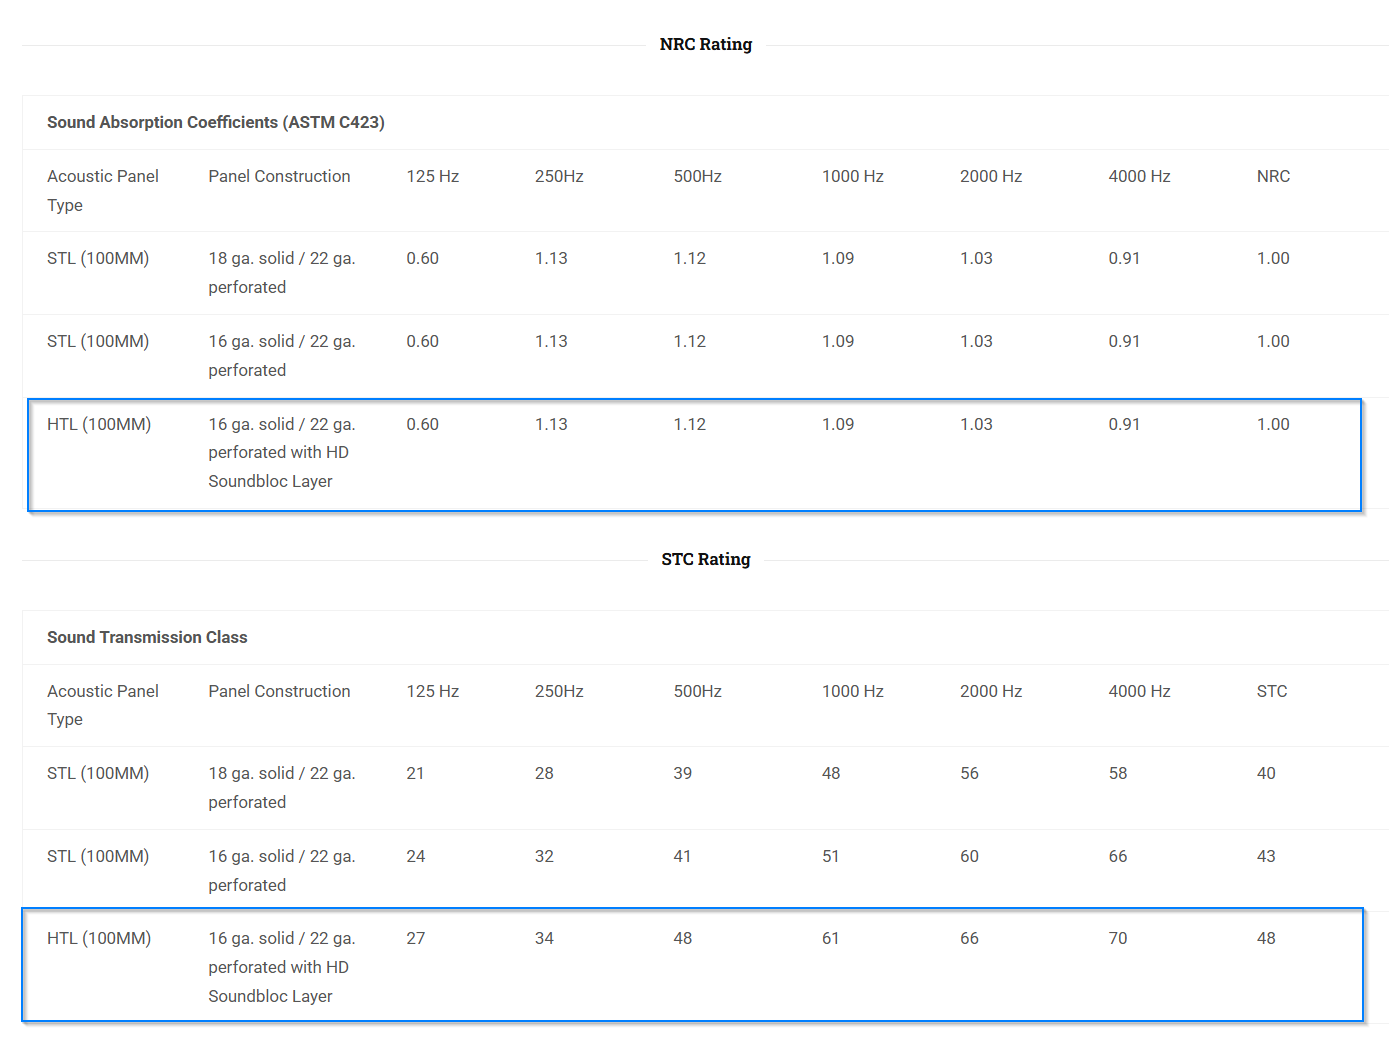
\includegraphics[scale=0.5]{Q5 AW Data.png}
    \caption{HTL (100MM) data from Acoustics World.}
    \label{figure:q5AWcaseData}
\end{figure}

\begin{figure}[htbp]
    \center
    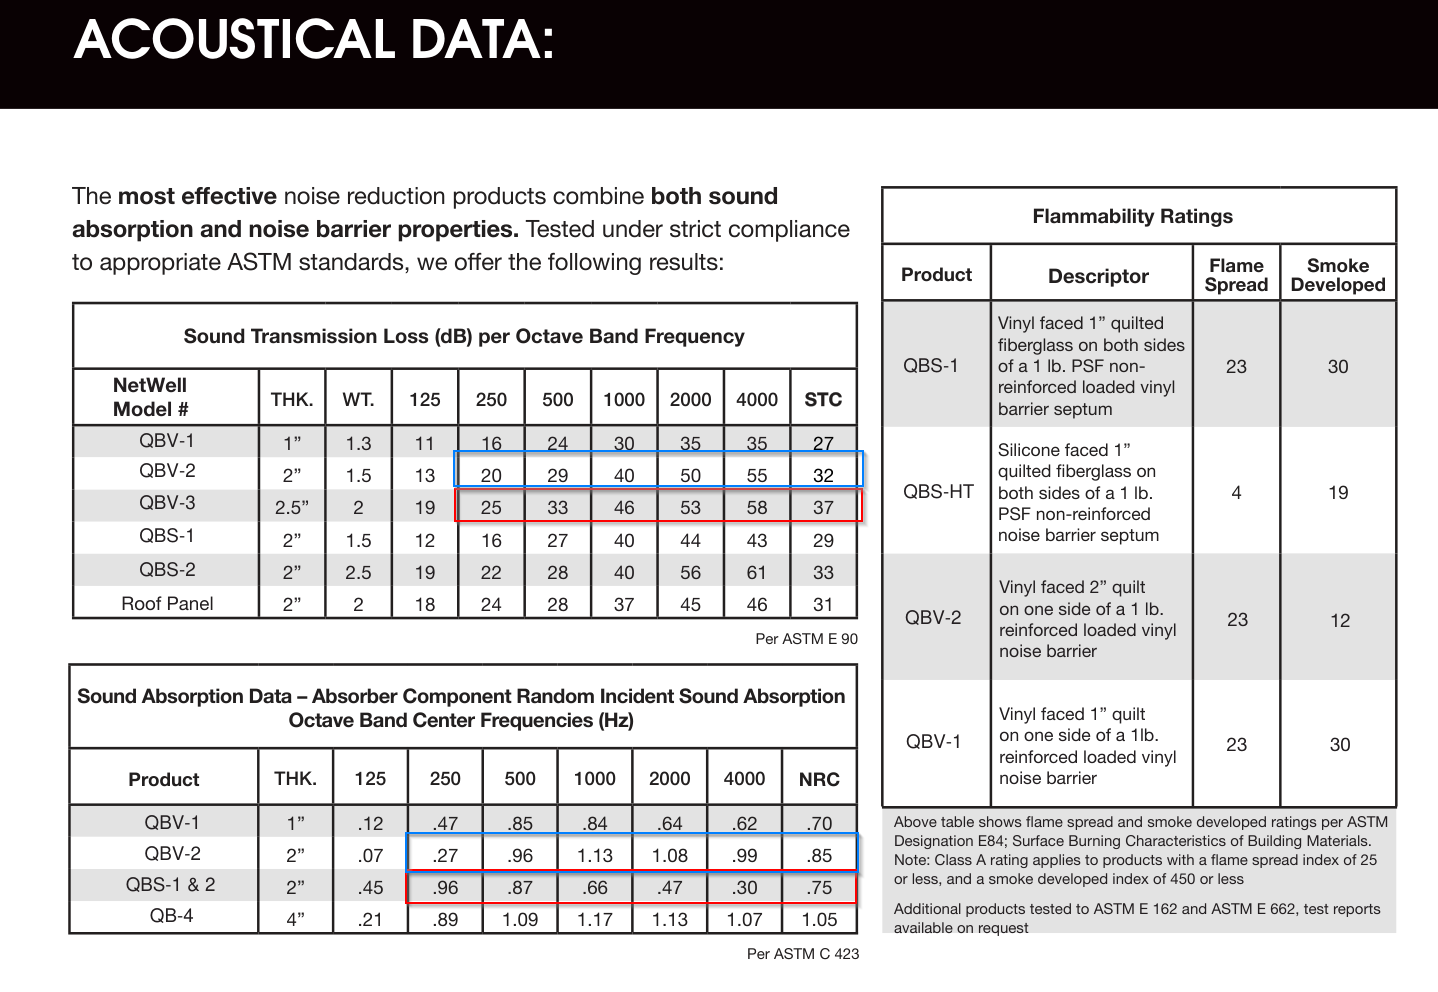
\includegraphics[scale=0.5]{Q5 NW Data.png}
    \caption{QBV-2 and QBV-3 data from Control Noise.}
    \label{figure:q5CNcaseData}
\end{figure}






\newpage
\section*{Problem 6 - Close-fitting Enclosure Design}

% For the insertion loss to be high, we need:
%
%   1.)  Compliance of the air to be high;  volume of enclosure must be large.
%   2.)  Compliance of each enclosure wall to be low;  low area, high stiffness, edges clamped).
%           AREA IS THE DOMINATE FACTOR OVER VOLUME.


The Matlab code for this problem is listed in Appendix~\ref{appendix:problem6}.

\vspace{0.25cm}
The required target insertion loss is 13 dB.  This is estimated with the given data and the assumption that the sound measurement distance is beyond the critical distance (i.e., in the diffuse field).


\vspace{0.25cm}
Table~\ref{table:Q6enclosureDesign} lists the dimensions of the designed enclosure.

\vspace{0.25cm}
\setlength{\abovecaptionskip}{0pt}
\vspace{0.1cm}
{\renewcommand{\arraystretch}{1.25}
\begin{table}[h!]
    \begin{center}
        \small
        \begin{tabular}{ | c | c | c | }
            \hline
            \textbf{Height [m]}  &  \textbf{Width [m]}  &  \textbf{Depth [m]}  \\
            \hline
            3  &  1.25 &  1.5  \\
            \hline
        \end{tabular}
    \end{center}
    \caption{Dimensions of the designed enclosure.}
    \label{table:Q6enclosureDesign}
\end{table}


Table~\ref{table:DesignParametersEnclosure} lists the design parameters for the design enclosure.

\vspace{0.25cm}
\setlength{\abovecaptionskip}{0pt}
\vspace{0.1cm}
{\renewcommand{\arraystretch}{1.25}
\begin{table}[h!]
    \begin{center}
        \small
        \begin{tabular}{ | c | c | c | c | c | c | c | }
            \hline
            \textbf{Wall}  &  \textbf{Width [m]}  &  \textbf{Height [m]}  &  \textbf{Area [$\mathbf m^2$]}  &  \textbf{Aspect Ratio}  &  \textbf{Correction}  &  \textbf{Compliance [$\frac{m^3\cdot s^2}{kg}$]}  \\
            \hline
            Top     &  1.25  &  1.5  &  1.875  &  1.2   &  1.8  &  1.42e-6  \\
            \hline
            Side 1  &  1.5   &  3    &  4.5    &  2.0   &  0.6  &  2.57e-6  \\
            Side 2  &  1.5   &  3    &  4.5    &  2.0   &  0.6  &  2.57e-6  \\
            \hline
            Side 3  &  1.25   &  3    &  3.75    &  2.4   &  0.5  &  1.49e-6  \\
            Side 4  &  1.25   &  3    &  3.75    &  2.4   &  0.5  &  1.49e-6  \\
            \rowcolor{Gray}
            \hline
        \end{tabular}
    \end{center}
    \caption{Enclosure design summary.}
    \label{table:DesignParametersEnclosure}
\end{table}


The estimated insertion loss without the hole is 13.5 dB, which exceeds the target loss of 13.

\vspace{0.25cm}
The estimated insertion loss with the hole is 1.2 dB, based on the hole depth correction of Deng (1998).  The hole reduces the required insertion loss.  The intake silencer needs to provide 11.8 dB of insertion loss.






\newpage
\section{Appendix - Matlab Code for Problem 1}
\label{appendix:problem1}

\lstinputlisting[style=Matlab-editor, numbers=left, mlshowsectionrules, basicstyle=\scriptsize]{../ACS_547_Module_2_Question_1_Wednesday_February_12_2025.m}


\newpage
\section{Appendix - Matlab Code for Problem 2}
\label{appendix:problem2}

\lstinputlisting[style=Matlab-editor, numbers=left, mlshowsectionrules, basicstyle=\scriptsize]{../ACS_547_Module_2_Question_2_Wednesday_February_12_2025.m}


\newpage
\section{Appendix - Matlab Code for Problem 3}
\label{appendix:problem3}

\lstinputlisting[style=Matlab-editor, numbers=left, mlshowsectionrules, basicstyle=\scriptsize]{../ACS_547_Module_2_Question_3_Wednesday_February_12_2025.m}


\newpage
\section{Appendix - Matlab Code for Problem 4}
\label{appendix:problem4}

\lstinputlisting[style=Matlab-editor, numbers=left, mlshowsectionrules, basicstyle=\scriptsize]{../ACS_547_Module_2_Question_4_Wednesday_February_12_2025.m}


\newpage
\section{Appendix - Matlab Code for Problem 5}
\label{appendix:problem5}

\lstinputlisting[style=Matlab-editor, numbers=left, mlshowsectionrules, basicstyle=\scriptsize]{../ACS_547_Module_2_Question_5_Wednesday_February_12_2025.m}


\newpage
\section{Appendix - Matlab Code for Problem 6}
\label{appendix:problem6}

\lstinputlisting[style=Matlab-editor, numbers=left, mlshowsectionrules, basicstyle=\scriptsize]{../ACS_547_Module_2_Question_6_Wednesday_February_12_2025.m}






\end{document}


% Reference(s):

% https://tex.stackexchange.com/questions/180222/how-to-change-font-size-for-specific-lstlisting


































%Table~\ref{table:machNumbers} lists the Mach numbers for each pipe section.  The flow rate is 0.017462 $\frac{m^3}{s}$.
%
%\setlength{\abovecaptionskip}{0pt}
%\vspace{0.1cm}
%{\renewcommand{\arraystretch}{1.5}
%\begin{table}[h!]
%    \begin{center}
%        \small
%        \begin{tabular}{ | c | c | c | }
%            \hline
%            \textbf{Pipe}  &  \textbf{Area [}{$\mathbf m^2$}\textbf{]}  &  \textbf{Mach Number [unitless]}  \\
%            \hline
%                Inlet  &  0.000507  &  -0.10047  \\
%                \hline
%                \rowcolor{Gray}
%                Outlet  &  0.00811  &  -0.0062795  \\
%            \hline
%        \end{tabular}
%    \end{center}
%    \caption{Calculated Mach numbers.}
%    \label{table:machNumbers}
%\end{table}





%\vspace{0.25cm}
%Figure~\ref{figure:intakeSystem} shows the transmission loss profiles.


%\newpage
%Table~\ref{table:helmholzResonator} lists the dimensions of the lossy Helmholtz resonator for the 129 Hz notch.
%
%\setlength{\abovecaptionskip}{0pt}
%\vspace{0.1cm}
%{\renewcommand{\arraystretch}{1.5}
%\begin{table}[h!]
%    \begin{center}
%        \small
%        \begin{tabular}{ | l | c | }
%            \hline
%            \textbf{Item}  &  \textbf{Measure]}  \\
%            \hline
%                Cavity Diameter                 &  0.254 m  \\
%                \hline
%                \rowcolor{Gray}
%                Neck Diameter                   &  0.0254 m  \\
%                \hline
%                Neck Length                     &  0.127 m  \\
%                \hline
%                \rowcolor{Gray}
%                Neck Area                       &  0.5e-3 $m^2$  \\
%                \hline
%                Length Correction 1, $L_{o1}$   &  0.711 m  \\
%                \hline
%                \rowcolor{Gray}
%                Length Correction 2, $L_{o2}$   &  0.3 m  \\
%                \hline
%                Cavity Volume                   &  8.0e-5 $m^3$  \\
%                \hline
%                \rowcolor{Gray}
%                Q Factor   &  10  \\
%            \hline
%        \end{tabular}
%    \end{center}
%    \caption{Dimensions of the lossy Helmholtz resonator (see slide 15 of Lecture 3 notes).}
%    \label{table:helmholzResonator}
%\end{table}





